\documentclass[slidetop, mathserif, dvipsnames]{beamer}

% \mode<presentation>
% {
% 	\usetheme{Warsaw}
% 	\setbeamercovered{transparent}
% }

% \usepackage{caption}
\usepackage{subcaption}
\captionsetup{compatibility=false}

% \usepackage[dvipsnames]{xcolor}

\mode<presentation>{
	\usetheme{Berlin}
	\setbeamercovered{transparent}
	\usefonttheme{professionalfonts}
}

\usepackage{amsmath, amsfonts, amssymb}
\usepackage{mathrsfs,dsfont}

\newcommand{\norm}[1]{\left\|#1\right\|}
\newcommand{\suchthat}{-\hspace{-10pt}\ni\hspace{-10pt}-}


\AtBeginSection[]
{
   \begin{frame}
       \tableofcontents[currentsection]
   \end{frame}
}

\addtobeamertemplate{navigation symbols}{}{%
    \usebeamerfont{footline}%
    \usebeamercolor[fg]{footline}%
    \hspace{1em}%
    \insertframenumber/\inserttotalframenumber
}

%% want to use verbatim: \begin{frame}[fragile]

\title[OTA]{Introdoction to Optimal Transport Assignments for Object Detection}
\author[chy1010]{Chien, Hung-Yu}
\date{\today}

\begin{document}

\begin{frame}
	\titlepage
\end{frame}

\section[Outline]{}
\begin{frame}
	\frametitle{Outlines}
	\tableofcontents
\end{frame}

\section{Introduction: the Motivation of Label Assignments}

\begin{frame}
    \frametitle{Recall}
    Recall the talk on last Friday, YOLOX proposed by Megvii has the following features:
    \begin{enumerate}
        \item multiple image size input
        \item decoupled heads
        \item anchor-free
        \item multi-positives
        \item SimOTA (simplified version of Optimal Transport Assignment)
    \end{enumerate}

    \quad

    Today we'll focus on the OTA, optimal transport assignment.

\end{frame}

\begin{frame}
    \frametitle{Motivation}

    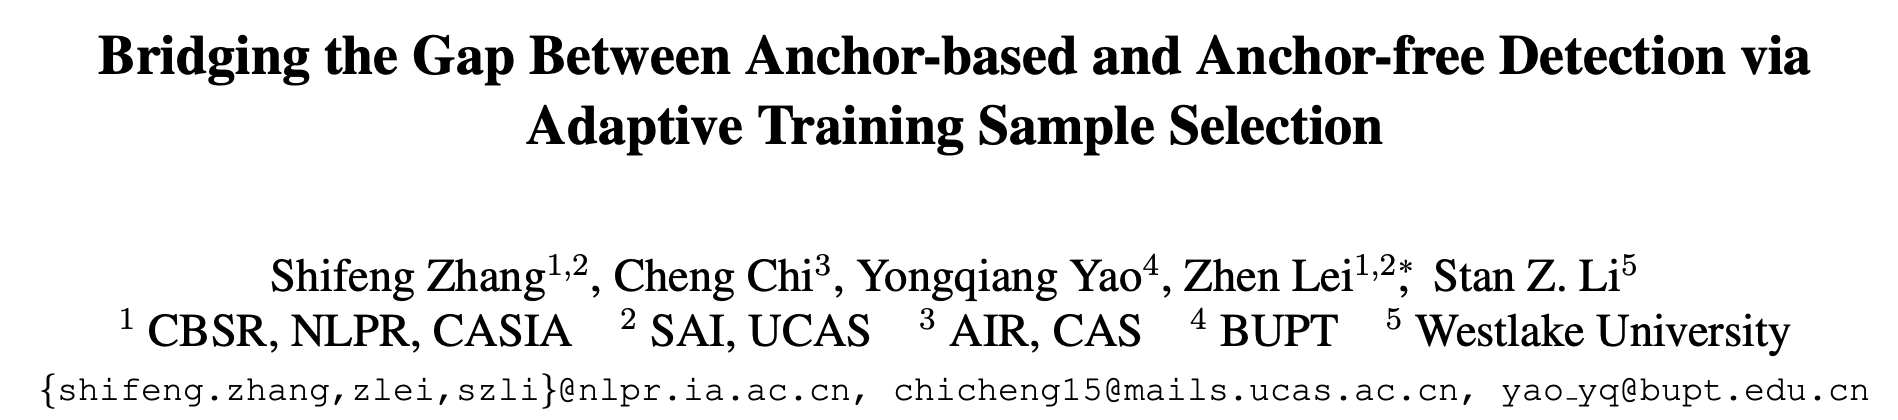
\includegraphics[width=300pt]{pics/atss_paper.png}

    \quad

    In these 2 to 3 years, anchor-free detectors have become popular
    due to the design of FPN and focal loss.
    However, in this CVPR 2020 paper (denoted by ATSS), the authors point out that:
    the {\bf essential difference} between the performance of these
    anchor-based and anchor-free detectors is actually
    {\bf how to define positive and negative trainng samples}.

\end{frame}

\begin{frame}
    \frametitle{Motivation}

    For usual detectors, since it is unknown that how many objects in an image,
    the RPN (region proposal networks) always makes dense predictions at each
    point on the feature map.

    \quad

    While at training, the {\bf imbalance} between ground-truth objects and dense
    sampling of possible object locations has trailed the accuracies.

    \quad

    In 2017, Focal loss is originally designed to address the extreme imbalance between
    {\bf fore- and back-ground classes} during training.
    In particular, the easily classified backgrounds comprise the majority.
    This focal loss aims to 
    {\bf down-weight these easy samples} and thus
    {\bf focus on training hard samples}.
\end{frame}

\begin{frame}
    \frametitle{Motivation}

    As focal loss try to alleviate the gradients from dominant easy samples,
    the core problem is still to divide the proposals into the following
    classes:
    \begin{itemize}
        \item positive samples: some object exists in this proposal.
            Need to train the classifier and regressor of anchor's offsets.
        \item negative samples: no object, or belong to the background class.
            Need to train the classifier to output 0 or the background class.
        \item ignore samples: not involed in training process.
    \end{itemize}

    Here we use `label assigment' to mention the association among
    proposals and ground-truth objects in training process.
\end{frame}

\begin{frame}
    \frametitle{Motivation}

    Back to the paper ATSS, they align the anchor-based 
    and anchor-free detectors by using the same tricks:

    \begin{figure}
    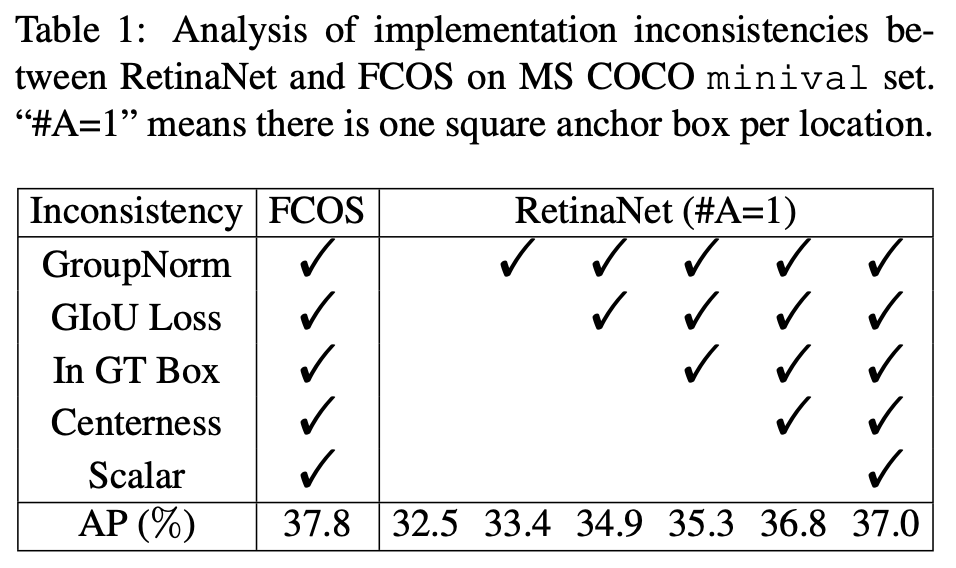
\includegraphics[width=150pt]{pics/atss_compare.png}
    \end{figure}

    Also, on each point of feature map, set $\#A=1$ means
    to use a single squared box to be an anchor.
    This is aim to compare an anchor point and an anchor box directly.

    % Scalar here means for different feature levels of FPN,
    % the regression values are in fact in different scales.
    % As a result, instead of using the standard exp(x),
    % for the feature level P_i, using exp(s_ix) with a trainable 
    % scalar s_i to automatically adjust the output.

\end{frame}

\begin{frame}
    \frametitle{Motivation}

    Hence the rest {\bf essential differences} are
    \begin{enumerate}
        \item the way to define positive and negative samples: Use IoU threholds (RetinaNet),
            use spatial constraints (F-COS).
        \item the regression starting from an `anchor box` (RetinaNet)
              or an `anchor point` (F-COS).
    \end{enumerate}

    \begin{figure}
    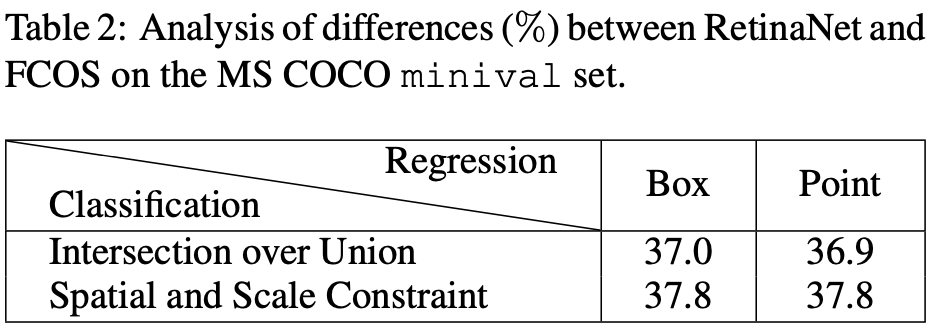
\includegraphics[width=150pt]{pics/atss_compare2.png}
    \end{figure}
    From the table in ATSS, we can see that the main difference
    is the way to define positive and negative samples.

\end{frame}

\section{Methods to Do Assignments}

\begin{frame}
    \frametitle{Assignments for Anchor-based Detector}

    For anchor-based detectors, the selection of positive and negative samples
    is often determined by the IoU of anchors and ground-truth objects.

    \begin{itemize}
    \item RPN in Faster R-CNN uses $0.7$ and $0.3$ as the thresholds for positive
        and negative samples.
    \item The R-CNN module uses $0.5$ as the pos/neg division.
    \end{itemize}
    This setting is widely used in Faster R-CNN's variants.
    % This kind of label assignments is proved effective and soon been adopted by
    % Faster R-CNN's variants and many one-stage detectors.

    Moreover, while the positive samples are still much more than ground truths,
    only a limited number of them are randomly chosen in the calculations of
    gradient descents.

\end{frame}

\begin{frame}
    \frametitle{Assignments for Anchor-free Detector}

    On the other side, anchor-free detectors such as FCOS, Foveabox, and etc.,
    assign positive samples if the location of the anchor point lies in
    \begin{enumerate}
    \item a ground truth bounding box (F-COS);
    \item or a shrunk version of it (Foveabox).
    \end{enumerate}

    \quad

    Furthermore, for another stream of anchor-free models:
    CornerNet, CenterNet, and etc., these models view objects as a point or
    a set of keypoints and hence have distinct characteristics from other
    detectors. We will not discussed this kind of models here.
    
\end{frame}


\begin{frame}
    \frametitle{Dynamic Assignments}

    The label assignment mentioned above are determined by fixed thresholds
    or spatial relations among dense predictions and ground truth objects.

    \quad

    Aiming to improve the assigning procedure, many methods are developed
    to produce anchor boxes / anchor points in more fancy ways:
    {\bf GuidedAnchoring}, {\bf MetaAnchor}, {\bf NoisyAnchors},
    {\bf FreeAnchor}, {\bf ATSS}, {\bf PAA}, {\bf AutoAssign} and etc.
    (We just list some of them here.)

    \quad

    As an example, for every ground truth, ATSS select $k$ anchors the most
    close to it. And calculate the {\tt mean} and {\tt std} of all IoU's.
    Then use {\tt mean$+$std} as the new threshold.

\end{frame}

\section{Optimal Transport Assignment}

\begin{frame}
    \frametitle{Further Idea for Label Assignment}

    Most of the label assignment methods explore the optimal assigning strategy
    for indivisual ground truth objects.
    But this failing to consider context information from a global perspective.

    \quad

    DeTR is the first work that attempts to consider label assignment from
    global view. By using Hungarian algorithm,
    an optimal bipartite matching between predictions
    and ground truth objects is made and the minimal loss in this iteration
    is obtained.

    \quad

    Why the global perspective is important?
    When the ground truths are crowded, there may be some ambiguous
    anchors which are hard to distribute to ground truth
    objects in the neighborhood.

\end{frame}

\begin{frame}
    \frametitle{Further Idea for Label Assignment}

    \begin{figure}
    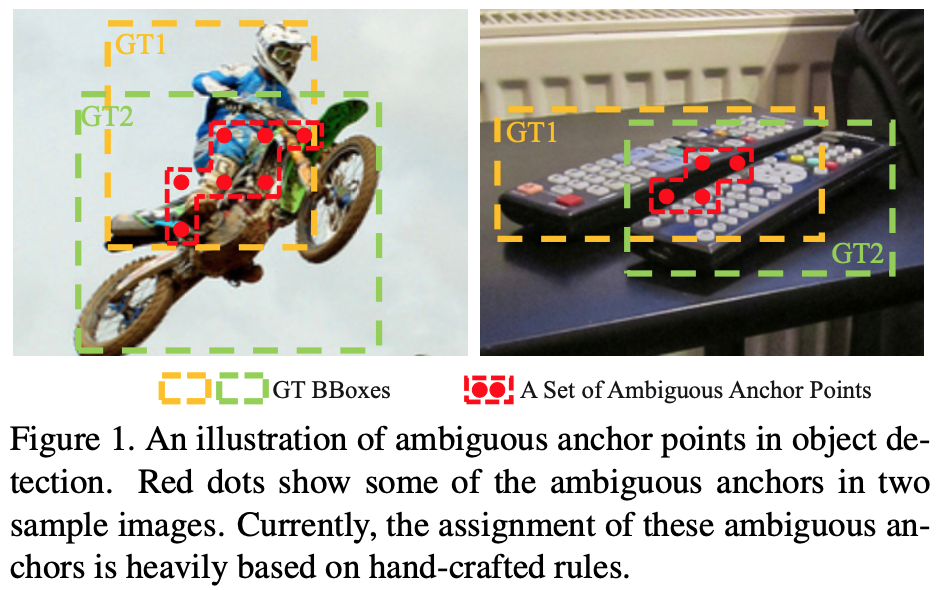
\includegraphics[width=200pt]{pics/ota_motivation.png}
    \end{figure}

    For this anchor-free detector, the anchor points which lie in the two
    ground truth boxes might be assigned as positive samples to
    only one ground-truth objects.

\end{frame}

\begin{frame}
    \frametitle{Optimal Transport Assignments}

    Unlike DeTR, for CNN-based detectors, the networks often produce several
    regions around a ground truth.
    Hence each ground truth object is likely to be assigned mutiple anchors
    to train. And this also helps the \underline{training efficiency}.

    \quad

    Therefore, by extending the idea of using Hungarian algorithm,
    the {\bf optimal transport assignment} is proposed
    to achieve the global optimal assignment under these one-to-many situations.

    \quad 

    Now in a one-to-many manner, we see each gt label as a supplier and each
    anchor a demander.
    Later we will introduce this problem again in an optimal transport's form.

\end{frame}

\begin{frame}
    \frametitle{What is OT (optimal transport)?}

    Suppose there are $m$ suppliers and $n$ demanders. The $i$-th supplier
    holds $s_i$ units of goods and $j$-th demander needs $d_j$ units of goods.
    Transporting cost of each unit of good from $i$-supplier to $j$-th demander
    is denoted by $c_{ij}$.
    The total ammounts are assumed equal: $\sum_{i}s_i = \sum_j d_j$.

    \quad
    
    The goal of this simplest OT problem is to find a {\bf transportation plan}
    $\pi^\star = \{\pi_{ij}\}$ to solve the minimization problem with constraints:
    \[
        \min_\pi\left\{\sum_{i,j} c_{ij}\pi_{ij}\ \left|\ \sum_i \pi_{ij} = d_j,~ \sum_j \pi_{ij}=s_i,~ \pi_{ij}\geq 0\right.\right\}.
    \]
    
\end{frame}

\end{document}